%--------------------------------------------------------------------------------
%--------------------------------------------------------------------------------
%--------------------------------------------------------------------------------

Ein Transistor besteht prinzipiell aus zwei PN-Übergängen, also zwei Dioden. 
Der Emitter-Basis Übergang ist üblicherweise (für einen Verstärkungsbetrieb) in Flussrichtung geschalten und der Basis-Kollektor Übergang in Sperrichtung. 

\subsection{Funktion von Bipolartransistoren \todo{1x}}\label{k6:bipolar}
Die folgenden Beschreibungen gelten immer für den npn Transistor (\autoref{fig:transistor-npn} wenn nicht anders erwähnt.    
    \begin{figure}
        \centering
        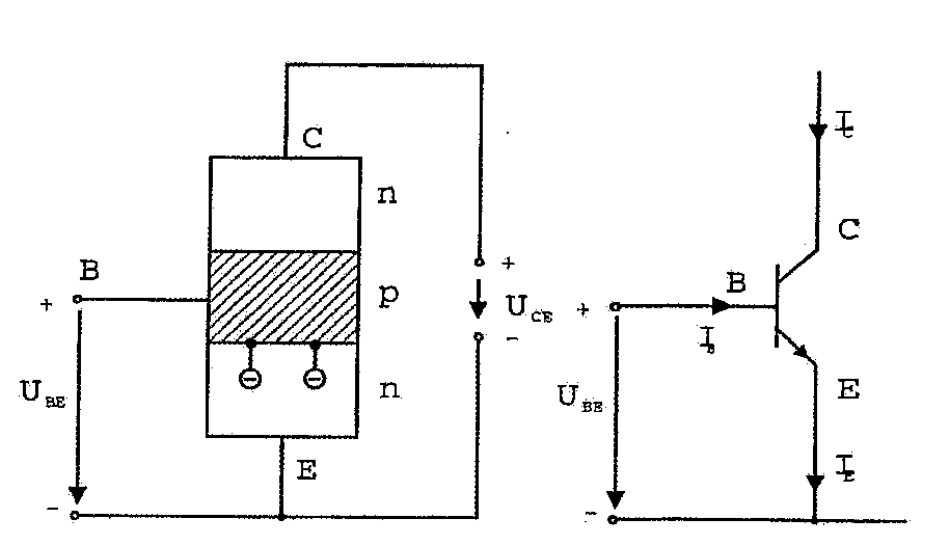
\includegraphics[width=0.66\textwidth]{fig/npn-transistor}
        \caption{NPN Bipolar Transistor}
        \label{fig:transistor-npn}
    \end{figure}
    
    \begin{figure}
        \centering
        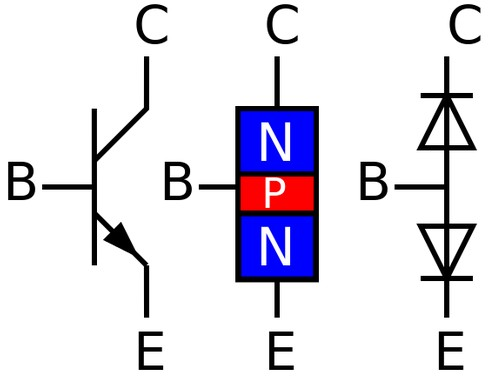
\includegraphics[width=0.66\textwidth]{fig/transistor-npn-diode.jpg}
        \caption{NPN Transistor und sein Diodenersatzschaltbild.}
        \label{fig:transistor-npn-diode}
    \end{figure}
    
    \subsubsection{Funktionionsweise}
    \emph{Sperre:} 
    
    \emph{Durchlass}
    
    Die vom Emitter in die Basis injizierten Elektronen werden von der Basis-Collector Raumladungszone abgesaugt und fließen \textit{nicht} über den Basisanschluss. 
    
    
    \subsubsection{Skizze}
    
    \begin{figure}
        \centering
        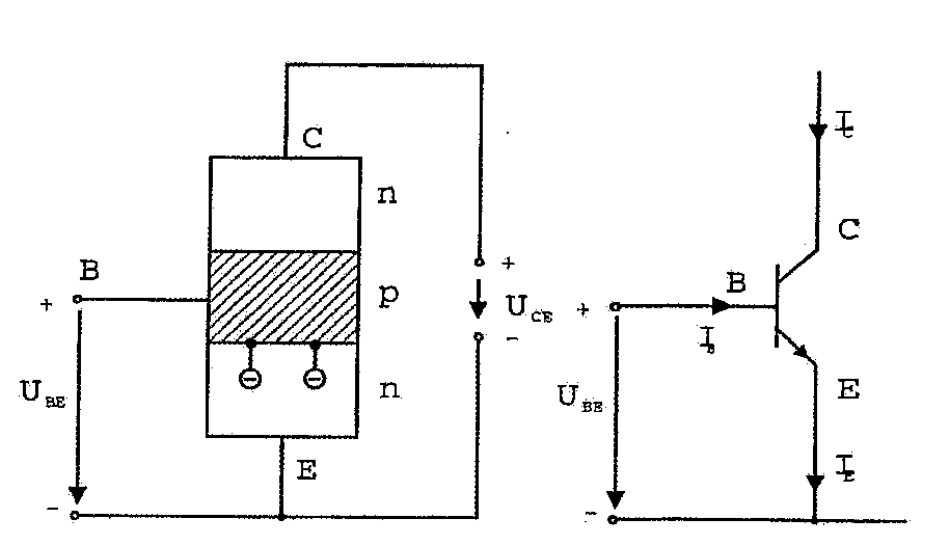
\includegraphics[width=0.66\textwidth]{fig/npn-transistor.jpg}
        \caption{Schematischer Aufbau und Schaltsymbol des npn-Transistors}
        \label{fig:npnTransistor}
    \end{figure}
    
    \begin{figure}
        \centering
        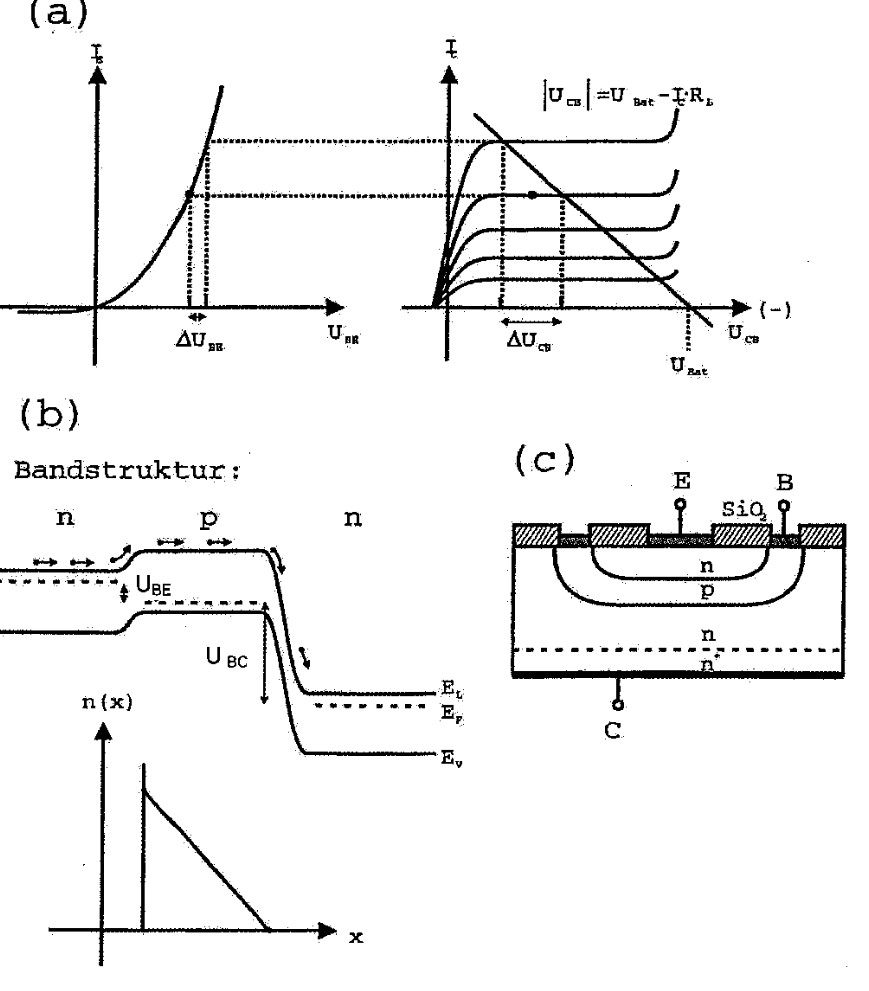
\includegraphics[width=0.66\textwidth]{fig/npn-transistor-kennlinien.jpg}
        \caption{Transistor - eine Hintereinanderschaltung zweier Dioden. Steile EB-Durchlasskennlinie steuer hochohmige EC-Diode. Weiters sind die Bandstruktur im Ort, der schematische AUfbau und das Diffusionsdreieck dargestellt.}
        \label{fig:npnTransistorKennlinie}
    \end{figure}
    
    \subsubsection{Warum wird er als Verst\"arker eingesetzt?}
\subsection{MOS-Struktur und Inversion \todo{2x}}\label{k6:mosInversion}

    \subsubsection{Wann spricht man von Inversion}
    \subsubsection{Leitungsband, Valenzband, Ef aufzeichnen}

\subsection{Diffusions-Dreieck beim Transistor \todo{0x}}\label{k6:diffusionsdreieck}
    \subsubsection{Warum fast linear?} exponential-Funktion im Ursprung ann\"ahernd linear
    \subsubsection{Was w\"are wenn die Basisl\"ange gr\"o{\ss}er als die Diffusionsl\"ange w\"are?} Man h\"atte die Wirkung von 2 Dioden und keinen Transistoreffekt mehr.

\subsection{Feldeffekt-Transistor \todo{0x}}\label{k6:fet}

\subsection{MOS-FET \todo{0x}}\label{k6:mosfet}
    \subsubsection{Aufbau}
    \subsubsection{Bandstruktur}

\subsection{MES-FET \todo{0x}}\label{k6:mesfet}

\subsection{Early-Effekt \todo{0x}}\label{k6:early}

\subsection{JFET \todo{0x}}\label{k6:jfet}
